%
% ---------------------------------------------------------------
% Copyright (C) 2012-2018 Gang Li
% ---------------------------------------------------------------
%
% This work is the default powerdot-tuliplab style test file and may be
% distributed and/or modified under the conditions of the LaTeX Project Public
% License, either version 1.3 of this license or (at your option) any later
% version. The latest version of this license is in
% http://www.latex-project.org/lppl.txt and version 1.3 or later is part of all
% distributions of LaTeX version 2003/12/01 or later.
%
% This work has the LPPL maintenance status "maintained".
%
% This Current Maintainer of this work is Gang Li.
%
%

\documentclass[
 size=14pt,
 paper=smartboard,  %a4paper, smartboard, screen
 mode=present, 		%present, handout, print
 display=slides, 	% slidesnotes, notes, slides
 style=tuliplab,  	% TULIP Lab style
 pauseslide,
 fleqn,leqno]{powerdot}


\usepackage{amssymb}
\usepackage{amsmath}
\usepackage{rotating}
\usepackage{graphicx}
\usepackage{boxedminipage}
\usepackage{media9}
\usepackage{rotate}
\usepackage{calc}
\usepackage[absolute]{textpos}
\usepackage{psfrag,overpic}
\usepackage{fouriernc}
\usepackage{pstricks,pst-node,pst-text,pst-3d,pst-grad}
\usepackage{moreverb,epsfig,subfigure}
\usepackage{pstricks}
\usepackage{pstricks-add}
\usepackage{pst-text}
\usepackage{pst-node, pst-tree}
\usepackage{booktabs}
\usepackage{etex}
\usepackage{breqn}
\usepackage{multirow}
\usepackage{gitinfo2}
\usepackage{xcolor}

\usepackage{todonotes}
% \usepackage{pst-rel-points}
\usepackage{animate}
\usepackage{fontawesome}

\usepackage{listings}
\lstset{frameround=fttt,
frame=trBL,
stringstyle=\ttfamily,
backgroundcolor=\color{yellow!20},
basicstyle=\footnotesize\ttfamily}
\lstnewenvironment{code}{
\lstset{frame=single,escapeinside=`',
backgroundcolor=\color{yellow!20},
basicstyle=\footnotesize\ttfamily}
}{}


\usepackage{hyperref}
\hypersetup{ % TODO: PDF meta Data
  pdftitle={Presentation Title},
  pdfauthor={Gang Li},
  pdfpagemode={FullScreen},
  pdfborder={0 0 0}
}


% \usepackage{auto-pst-pdf}
% package to show source code

\definecolor{LightGray}{rgb}{0.9,0.9,0.9}
\newlength{\pixel}\setlength\pixel{0.000714285714\slidewidth}
\setlength{\TPHorizModule}{\slidewidth}
\setlength{\TPVertModule}{\slideheight}
\newcommand\highlight[1]{\fbox{#1}}
\newcommand\icite[1]{{\footnotesize [#1]}}

\newcommand\twotonebox[2]{\fcolorbox{pdcolor2}{pdcolor2}
{#1\vphantom{#2}}\fcolorbox{pdcolor2}{white}{#2\vphantom{#1}}}
\newcommand\twotoneboxo[2]{\fcolorbox{pdcolor2}{pdcolor2}
{#1}\fcolorbox{pdcolor2}{white}{#2}}
\newcommand\vpspace[1]{\vphantom{\vspace{#1}}}
\newcommand\hpspace[1]{\hphantom{\hspace{#1}}}
\newcommand\COMMENT[1]{}

\newcommand\placepos[3]{\hbox to\z@{\kern#1
        \raisebox{-#2}[\z@][\z@]{#3}\hss}\ignorespaces}

\renewcommand{\baselinestretch}{1.2}


\newcommand{\draftnote}[3]{
	\todo[author=#2,color=#1!30,size=\footnotesize]{\textsf{#3}}	}
% TODO: add yourself here:
%
\newcommand{\gangli}[1]{\draftnote{blue}{GLi:}{#1}}
\newcommand{\shaoni}[1]{\draftnote{green}{sn:}{#1}}
\newcommand{\gliMarker}
	{\todo[author=GLi,size=\tiny,inline,color=blue!40]
	{Gang Li has worked up to here.}}
\newcommand{\snMarker}
	{\todo[author=Sn,size=\tiny,inline,color=green!40]
	{Shaoni has worked up to here.}}

%%%%%%%%%%%%%%%%%%%%%%%%%%%%%%%%%%%%%%%%%%%%%%%%%%%%%%%%%%%%%%%%%%%%%%%%
% title
% TODO: Customize to your Own Title, Name, Address
%
\title{Flip00 Project Final Test Presentation}
\author{
Shuxia Lin\\
SouthEast University
}
\date{\gitCommitterDate}


% Customize the setting of slides
\pdsetup{
% TODO: Customize the left footer, and right footer
rf=\href{http://www.tulip.org.au}{
Last Changed by: \textsc{\gitCommitterName}\ \gitVtagn-\gitAbbrevHash\ (\gitAuthorDate)
},
cf={Flip00 Project Final Test Presentation},
}


\begin{document}

\maketitle

%\begin{slide}{Overview}
%\tableofcontents[content=sections]
%\end{slide}


%%==========================================================================================
%%
\begin{slide}[toc=,bm=]{Overview}
\tableofcontents[content=currentsection,type=1]
\end{slide}
%%
%%==========================================================================================


\section{Problem Statement}


%%==========================================================================================
%%
\begin{slide}{Problem Definition}
\begin{center}
\twotonebox{\rotatebox{90}{Defn}}{\parbox{.96\textwidth}
{After a month of making scientific observations 
and taking careful measurements, 
can determined that 900 \textcolor{orange}{ghouls},
\textcolor{orange}{ghosts}, 
and \textcolor{orange}{goblins}.
The raw dataset contains train set with \textcolor{orange}{371} 
samples and \textcolor{orange}{529} unlabeled samples as test set.
Through the train data, find the relationship
between the attributes and species, 
and then identify the ghastly creatures in test data.
}}
\end{center}
\begin{center}
	
\includegraphics[width=.8\linewidth]{figures/bar.eps}
\end{center}
\end{slide}

%%==========================================================================================

\begin{slide}{Data Set}
\begin{center}
	\twotonebox{\rotatebox{90}{Defn}}{\parbox{.96\textwidth}
		{There are 4 numerical variables and 1 categorical,
			and no missing values.
			Numerical columns are either normalized or show a percentage, 
			so no need to scale them.
	}}
\end{center}
\begin{center}
	\begin{itemize}
		\item Data List
		\begin{description}
			\item[id] id of the creature
			\item[bone\_length] average length of bone in the creature, 
			normalized between \emph{0} and \emph{1}
			\item[rotting\_flesh] percentage of rotting flesh in the creature
			\item[hair\_length] average hair length, 
			normalized between \emph{0} and \emph{1}
			\item[has\_soul] percentage of soul in the creature
			\item[Color] dominant color of the creature: 
			\emph{white},\emph{black},\emph{clear},
			\emph{blue},\emph{green},\emph{blood}
			\item[type] target variable: 
			\emph{Ghost}, \emph{Goblin}, and \emph{Ghoul}
		\end{description}
		\item Train Data and Test Data
		\
		
		Divide the raw train set into train data 
		and test data, 
		and the ratio is 8:2. 		
	\end{itemize}
\end{center}
\end{slide}

%%==========================================================================================

\begin{slide}{Evaluation Methods}
\begin{center}
	\begin{itemize}
		\item F1 Score
		\item Precision
		\item Recall
		\item AUC
	\end{itemize}
\end{center}

\end{slide}

%%==========================================================================================

\section{Data Exploration}

%%==========================================================================================

\begin{slide}{Data Visualize}
\begin{center}
	\twotonebox{\rotatebox{90}{Exp}}{\parbox{.96\textwidth}
		{Use EDA to plot the distribution of the data,
			can observate the data intuitively and
			find the relation between the attribute values. 
	}}
\end{center}
\begin{center}
	\begin{itemize}
		\item Figures
		\begin{itemize}
			\item Histogrm
			\item Boxplot
			\item Pairplot
			\item Correllogram
		\end{itemize}
	\end{itemize}
\end{center}
\end{slide}
%%
%%==========================================================================================


%%==========================================================================================
%%
\begin{slide}[toc=,bm=]{Data Visualize}
	\begin{center}
		\twotonebox{\rotatebox{90}{Exp}}{\parbox{.96\textwidth}
			{It seems that all numerical features may be useful, 
				but many colors are evenly distributes among the monsters,
				which means they maybe have little effect on classification. 
		}}
	\end{center}
	
\begin{center}
	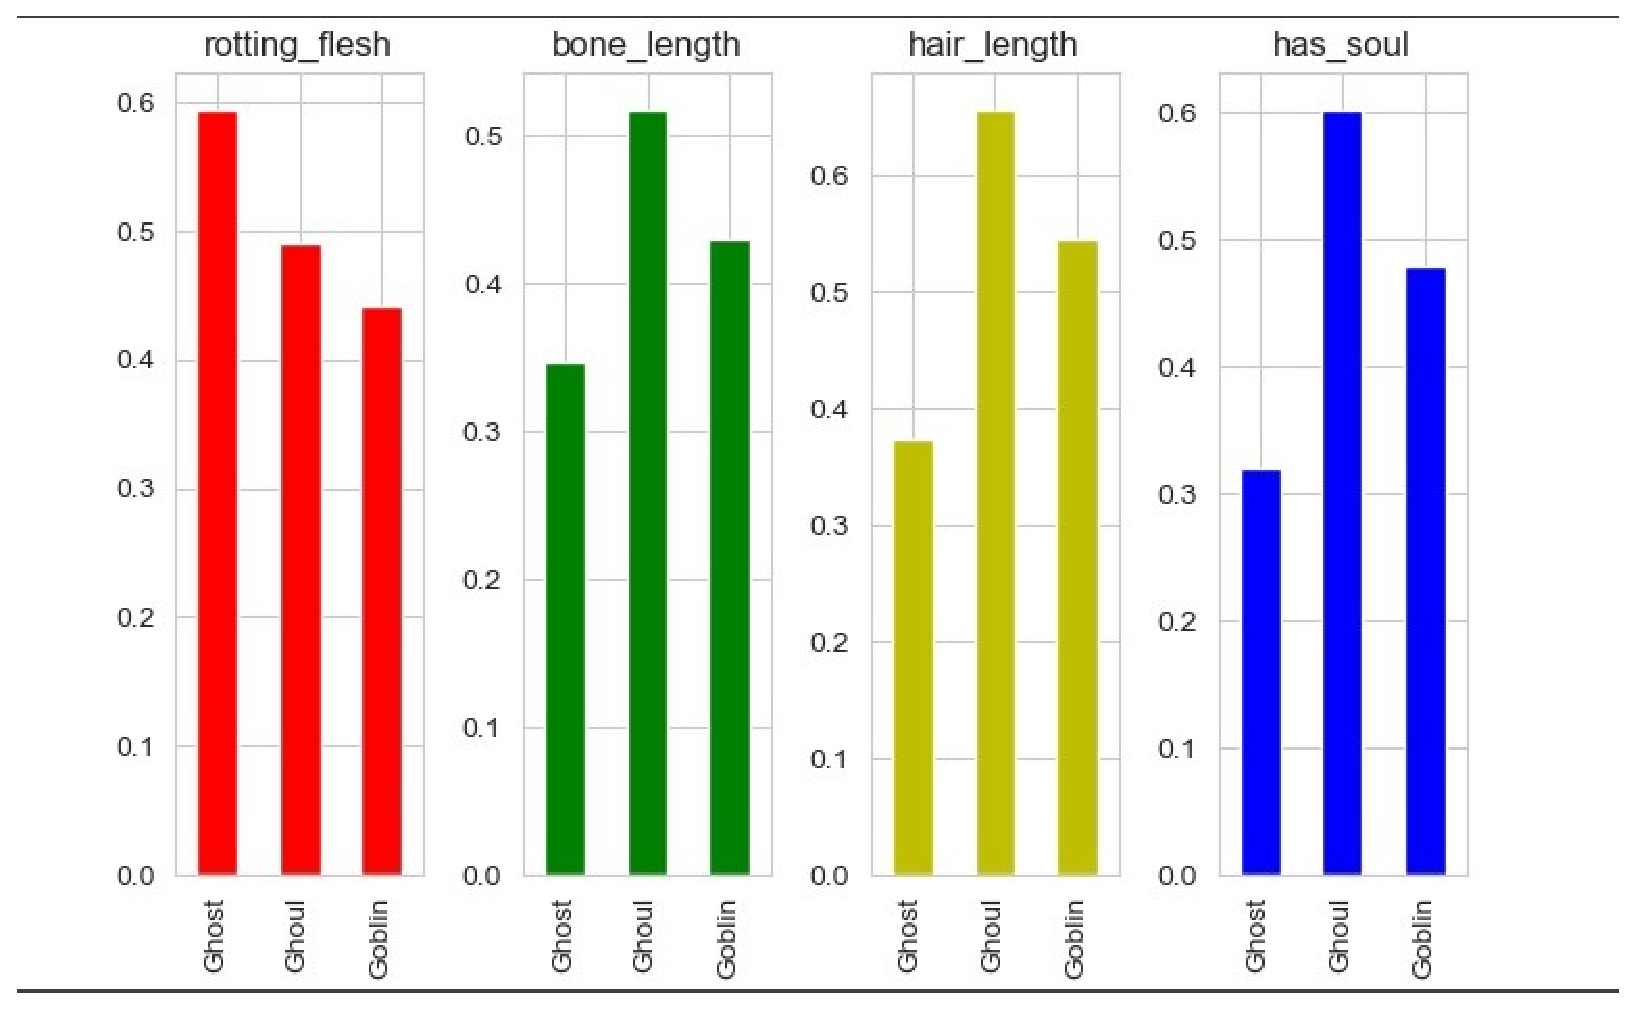
\includegraphics[width=.4\linewidth,height=.4\linewidth]{figures/his_1.eps}
	\quad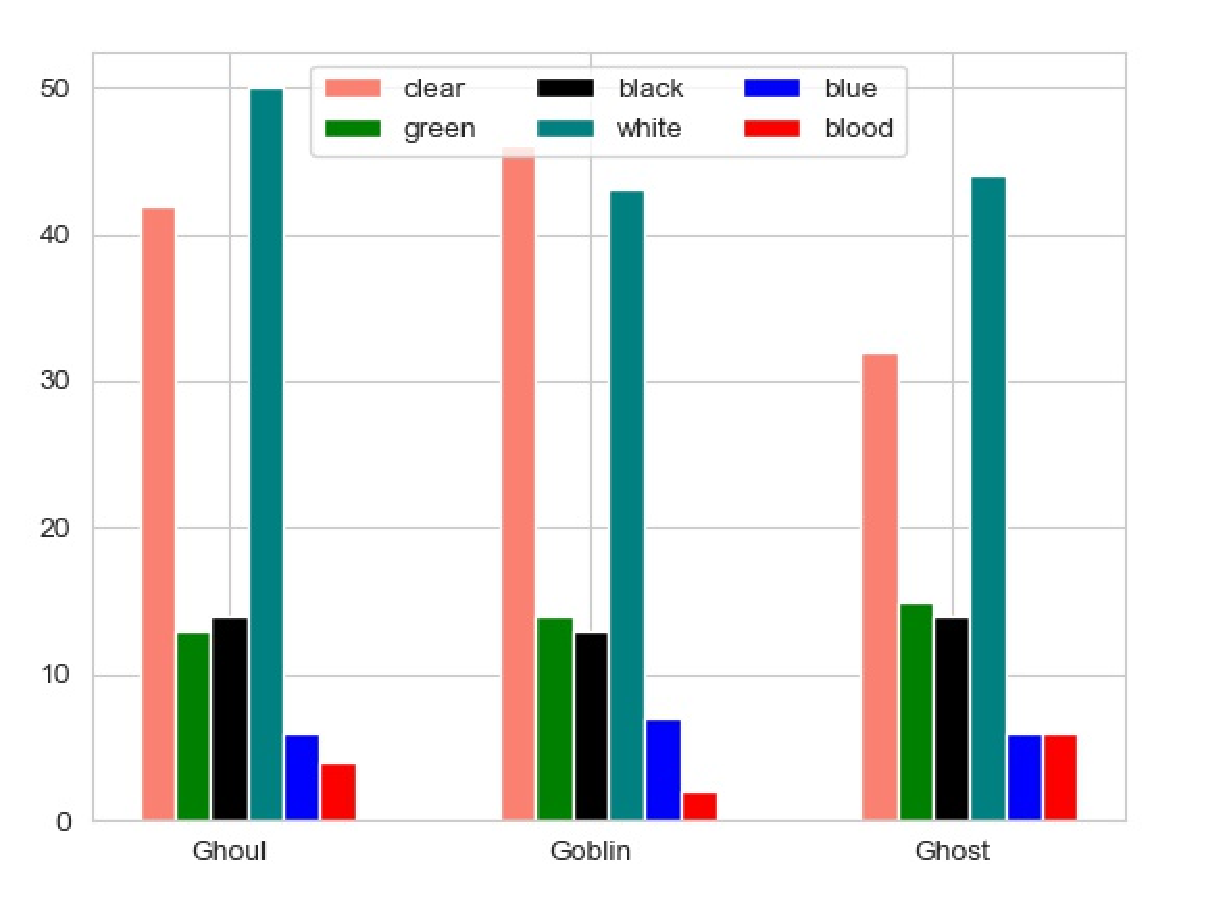
\includegraphics[width=.4\linewidth,height=.4\linewidth]{figures/his_2.eps}
\end{center}
\end{slide}
%%
%%==========================================================================================

\begin{slide}[toc=,bm=]{Data Visualize}
	\begin{center}
		\twotonebox{\rotatebox{90}{Exp}}{\parbox{.96\textwidth}
			{Based on the above observation on boxplot,
				we guess that the predictive accuracy of Ghost and Ghoul 
				will be better than Goblin.
				And the outliers are very small,
				which can be ignored. 
				As for correllogram, can find that it is 
				no obvious linear relationship 
				between these variables.
		}}
	\end{center}
	
	\begin{center}
		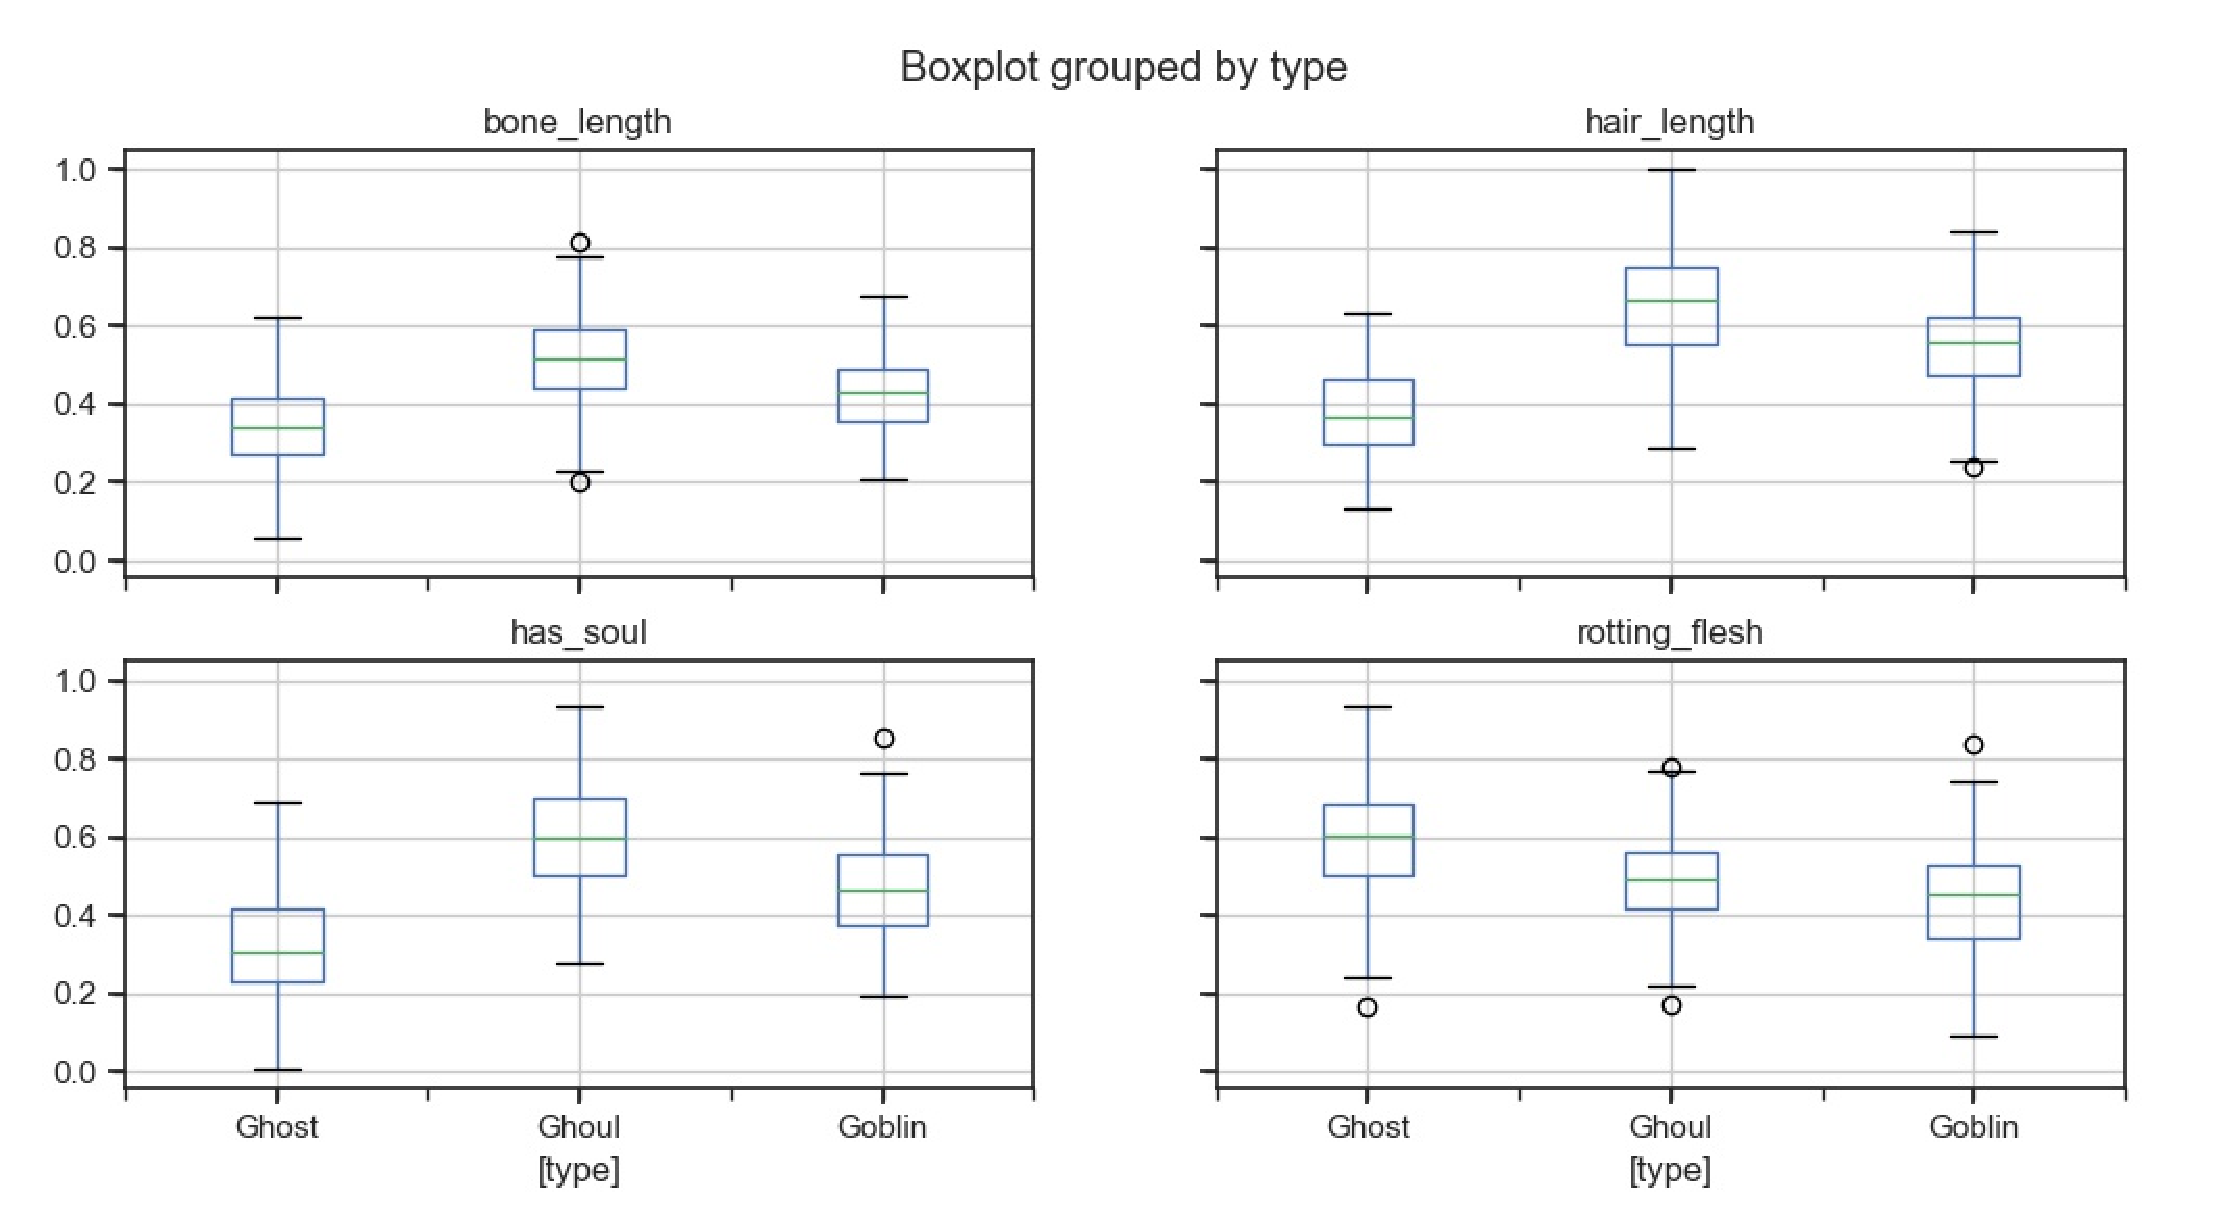
\includegraphics[width=.4\linewidth,height=.4\linewidth]{figures/boxplot.eps}
		\quad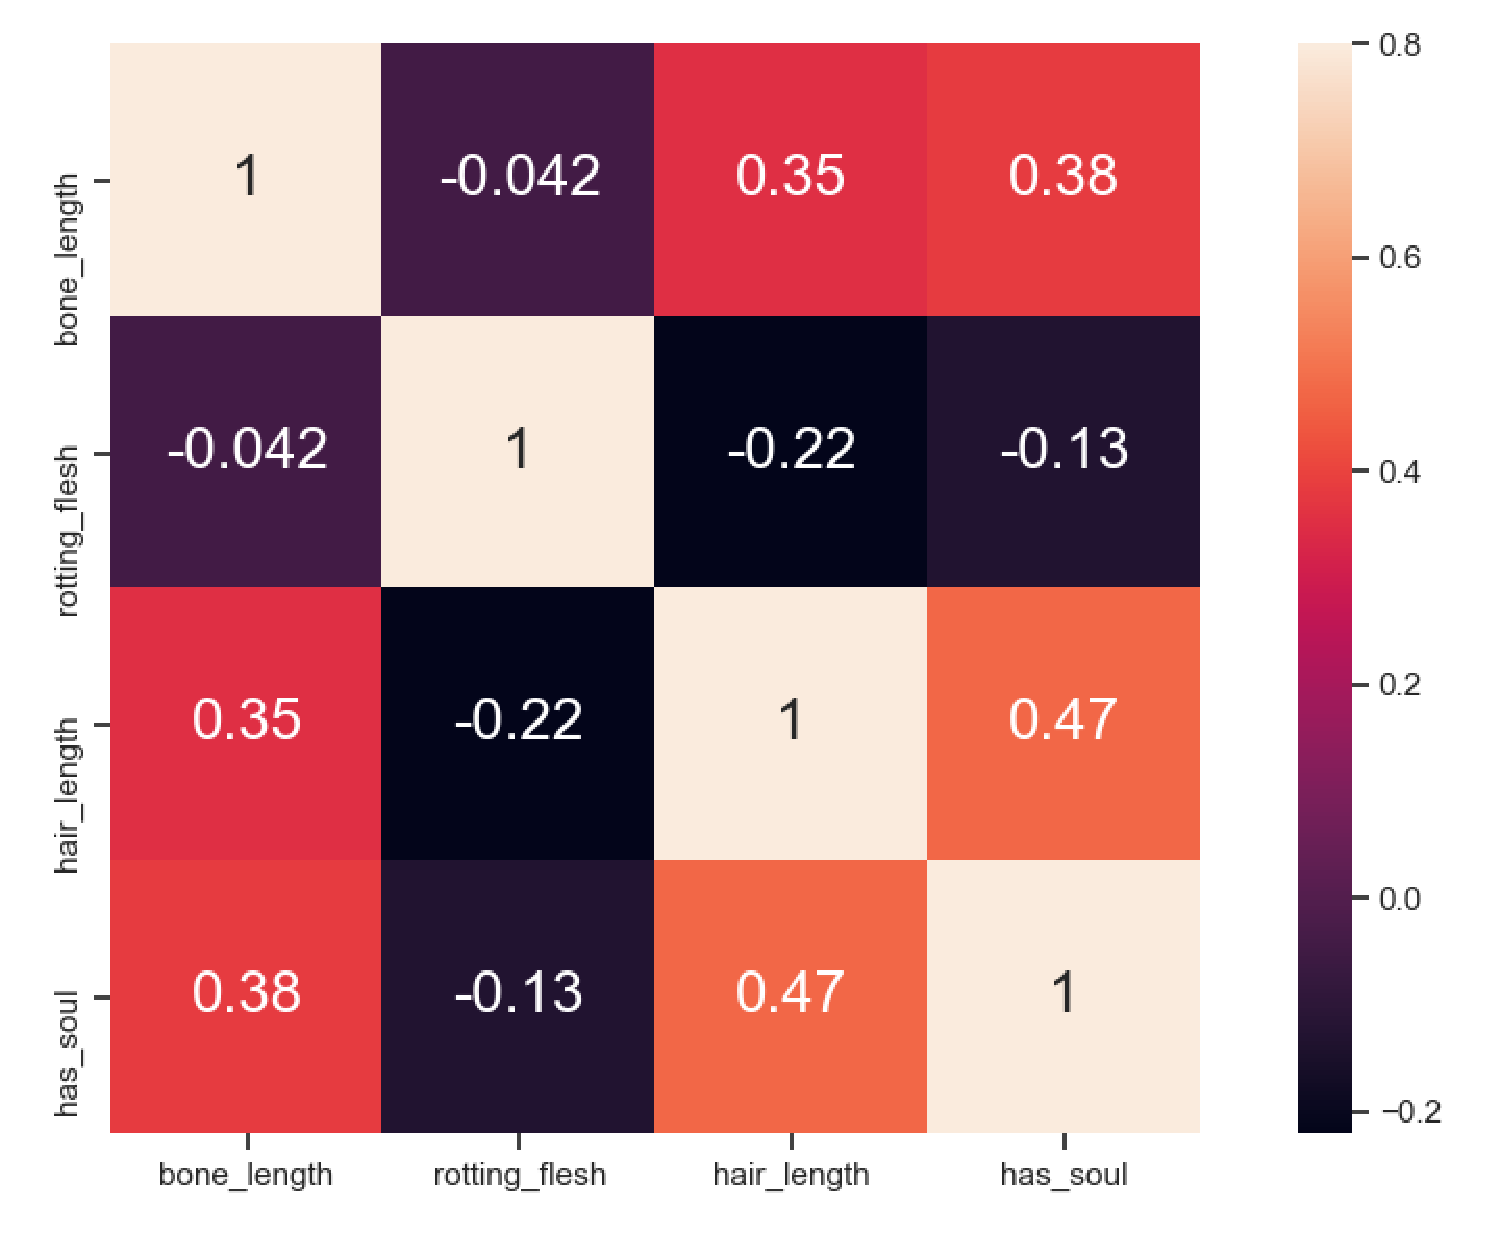
\includegraphics[width=.4\linewidth,height=.4\linewidth]{figures/corr.eps}	
	\end{center}
\end{slide}

%%==========================================================================================
%%

\begin{slide}[toc=,bm=]{Data Visualize}
	\begin{center}
		\twotonebox{\rotatebox{90}{Exp}}{\parbox{.96\textwidth}
			{This pairplot shows that 
				data is distributed normally. 
				And while most pairs are widely scattered 
				(in relationship to the type), 
				some of them show clusters: 
				hair\_length and has\_soul, 
				hair\_length and bone\_length. 
				So it may need to reassemble the data.
		}}
	\end{center}
	\begin{center}
		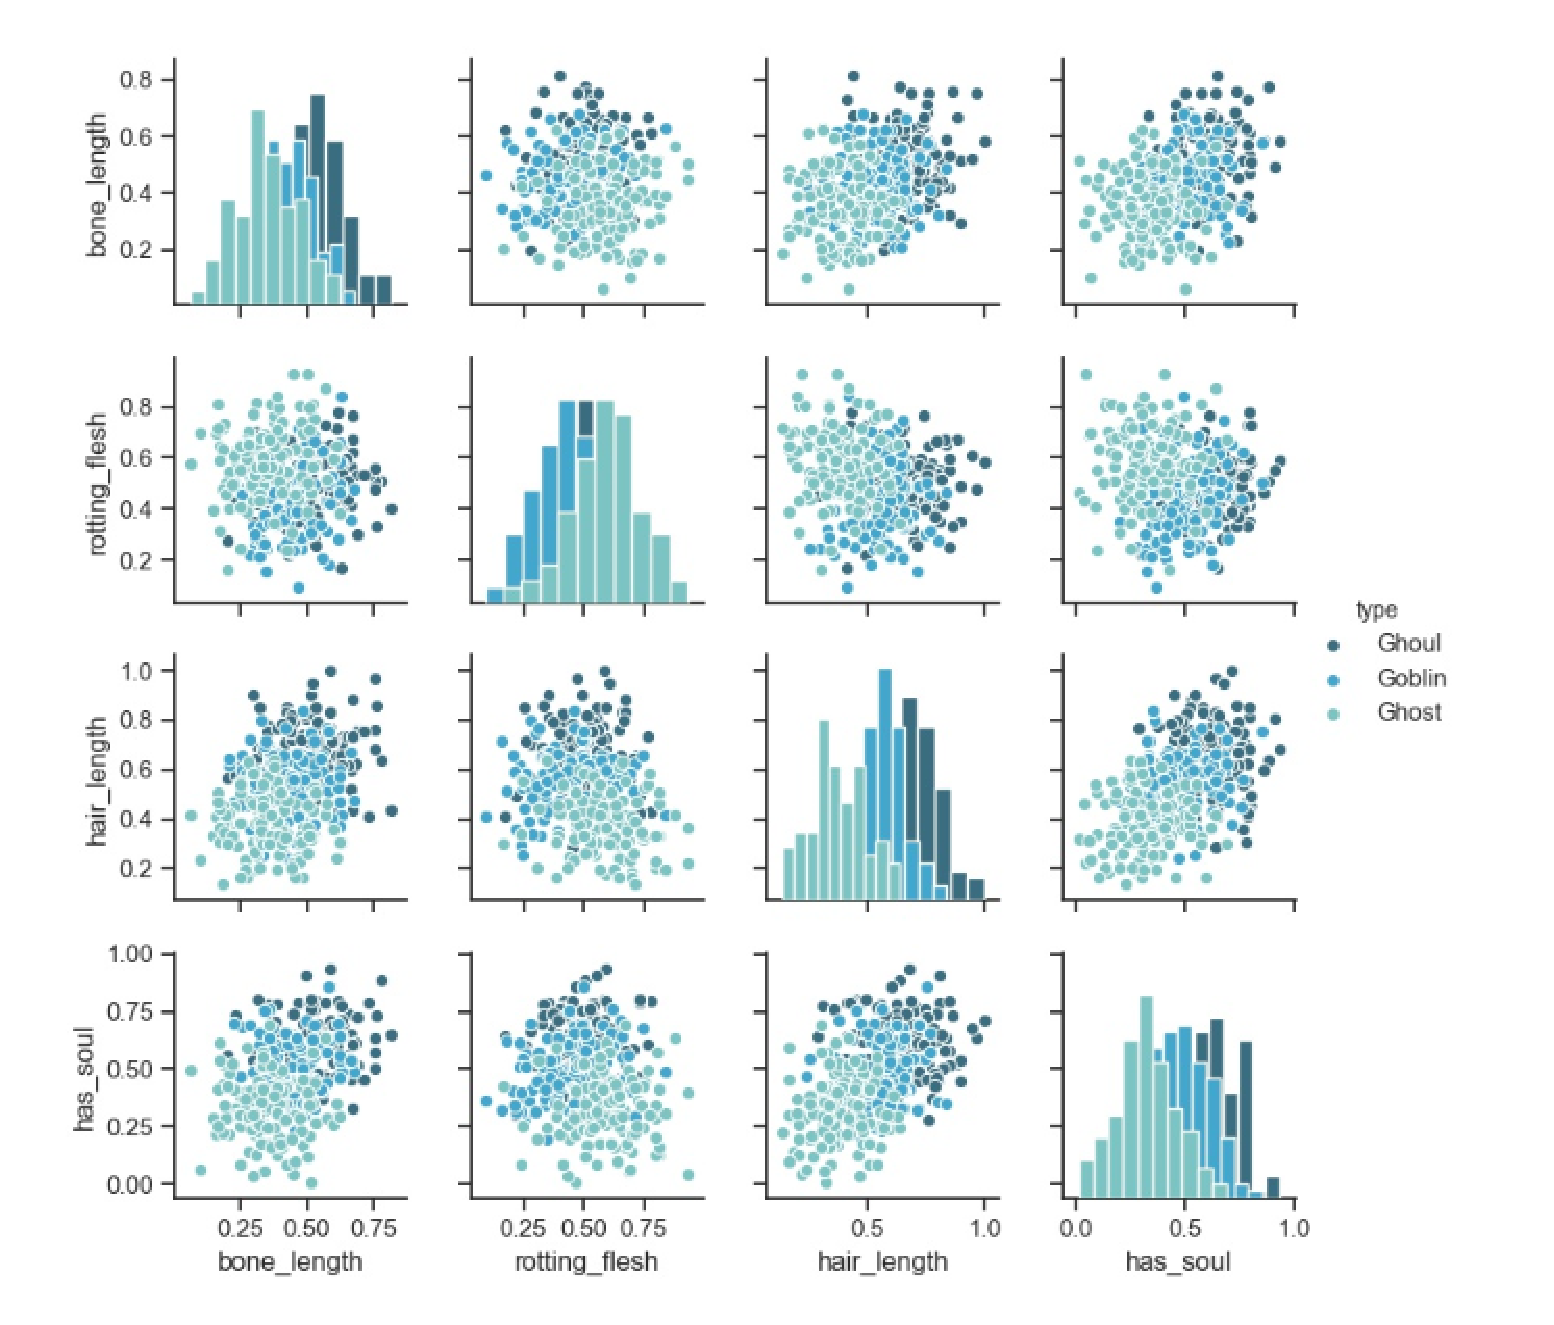
\includegraphics[width=.5\linewidth,height=.4\linewidth]{figures/pairplot.eps}	
	\end{center}
\end{slide}

%%==========================================================================================
%%
\begin{slide}{Data Engineering}
As it can be seen from 
the pairplot front 
the data is distributed normally. 
But some of them show clusters: 
hair\_length and has\_soul, 
hair\_length and bone\_length. 
So  create new variables 
with multiplication of these columns: 

\begin{center}
	\begin{itemize}
		\item New Features
		\
		\begin{description}
			\item[hair\_soul] row[hair\_length]*row[has\_soul] 
			\item[hair\_bone]  row[hair\_length]*row[bone\_length] 
			\item[bone\_soul]  row[bone\_length]*row[has\_soul] 
			\item[hair\_soul\_bone]  row[hair\_length]*row[has\_soul]*row[bone\_length] 
		\end{description}
	\end{itemize}
	
\end{center}

\end{slide}

%%=====================================================================

\begin{slide}[toc=,bm=]{Data Engineering}

Analyse the new features in a pairplot, 
it can be seen from the picture that 
there is a clear linear relationship 
between the variables. 
	
	\begin{center}
		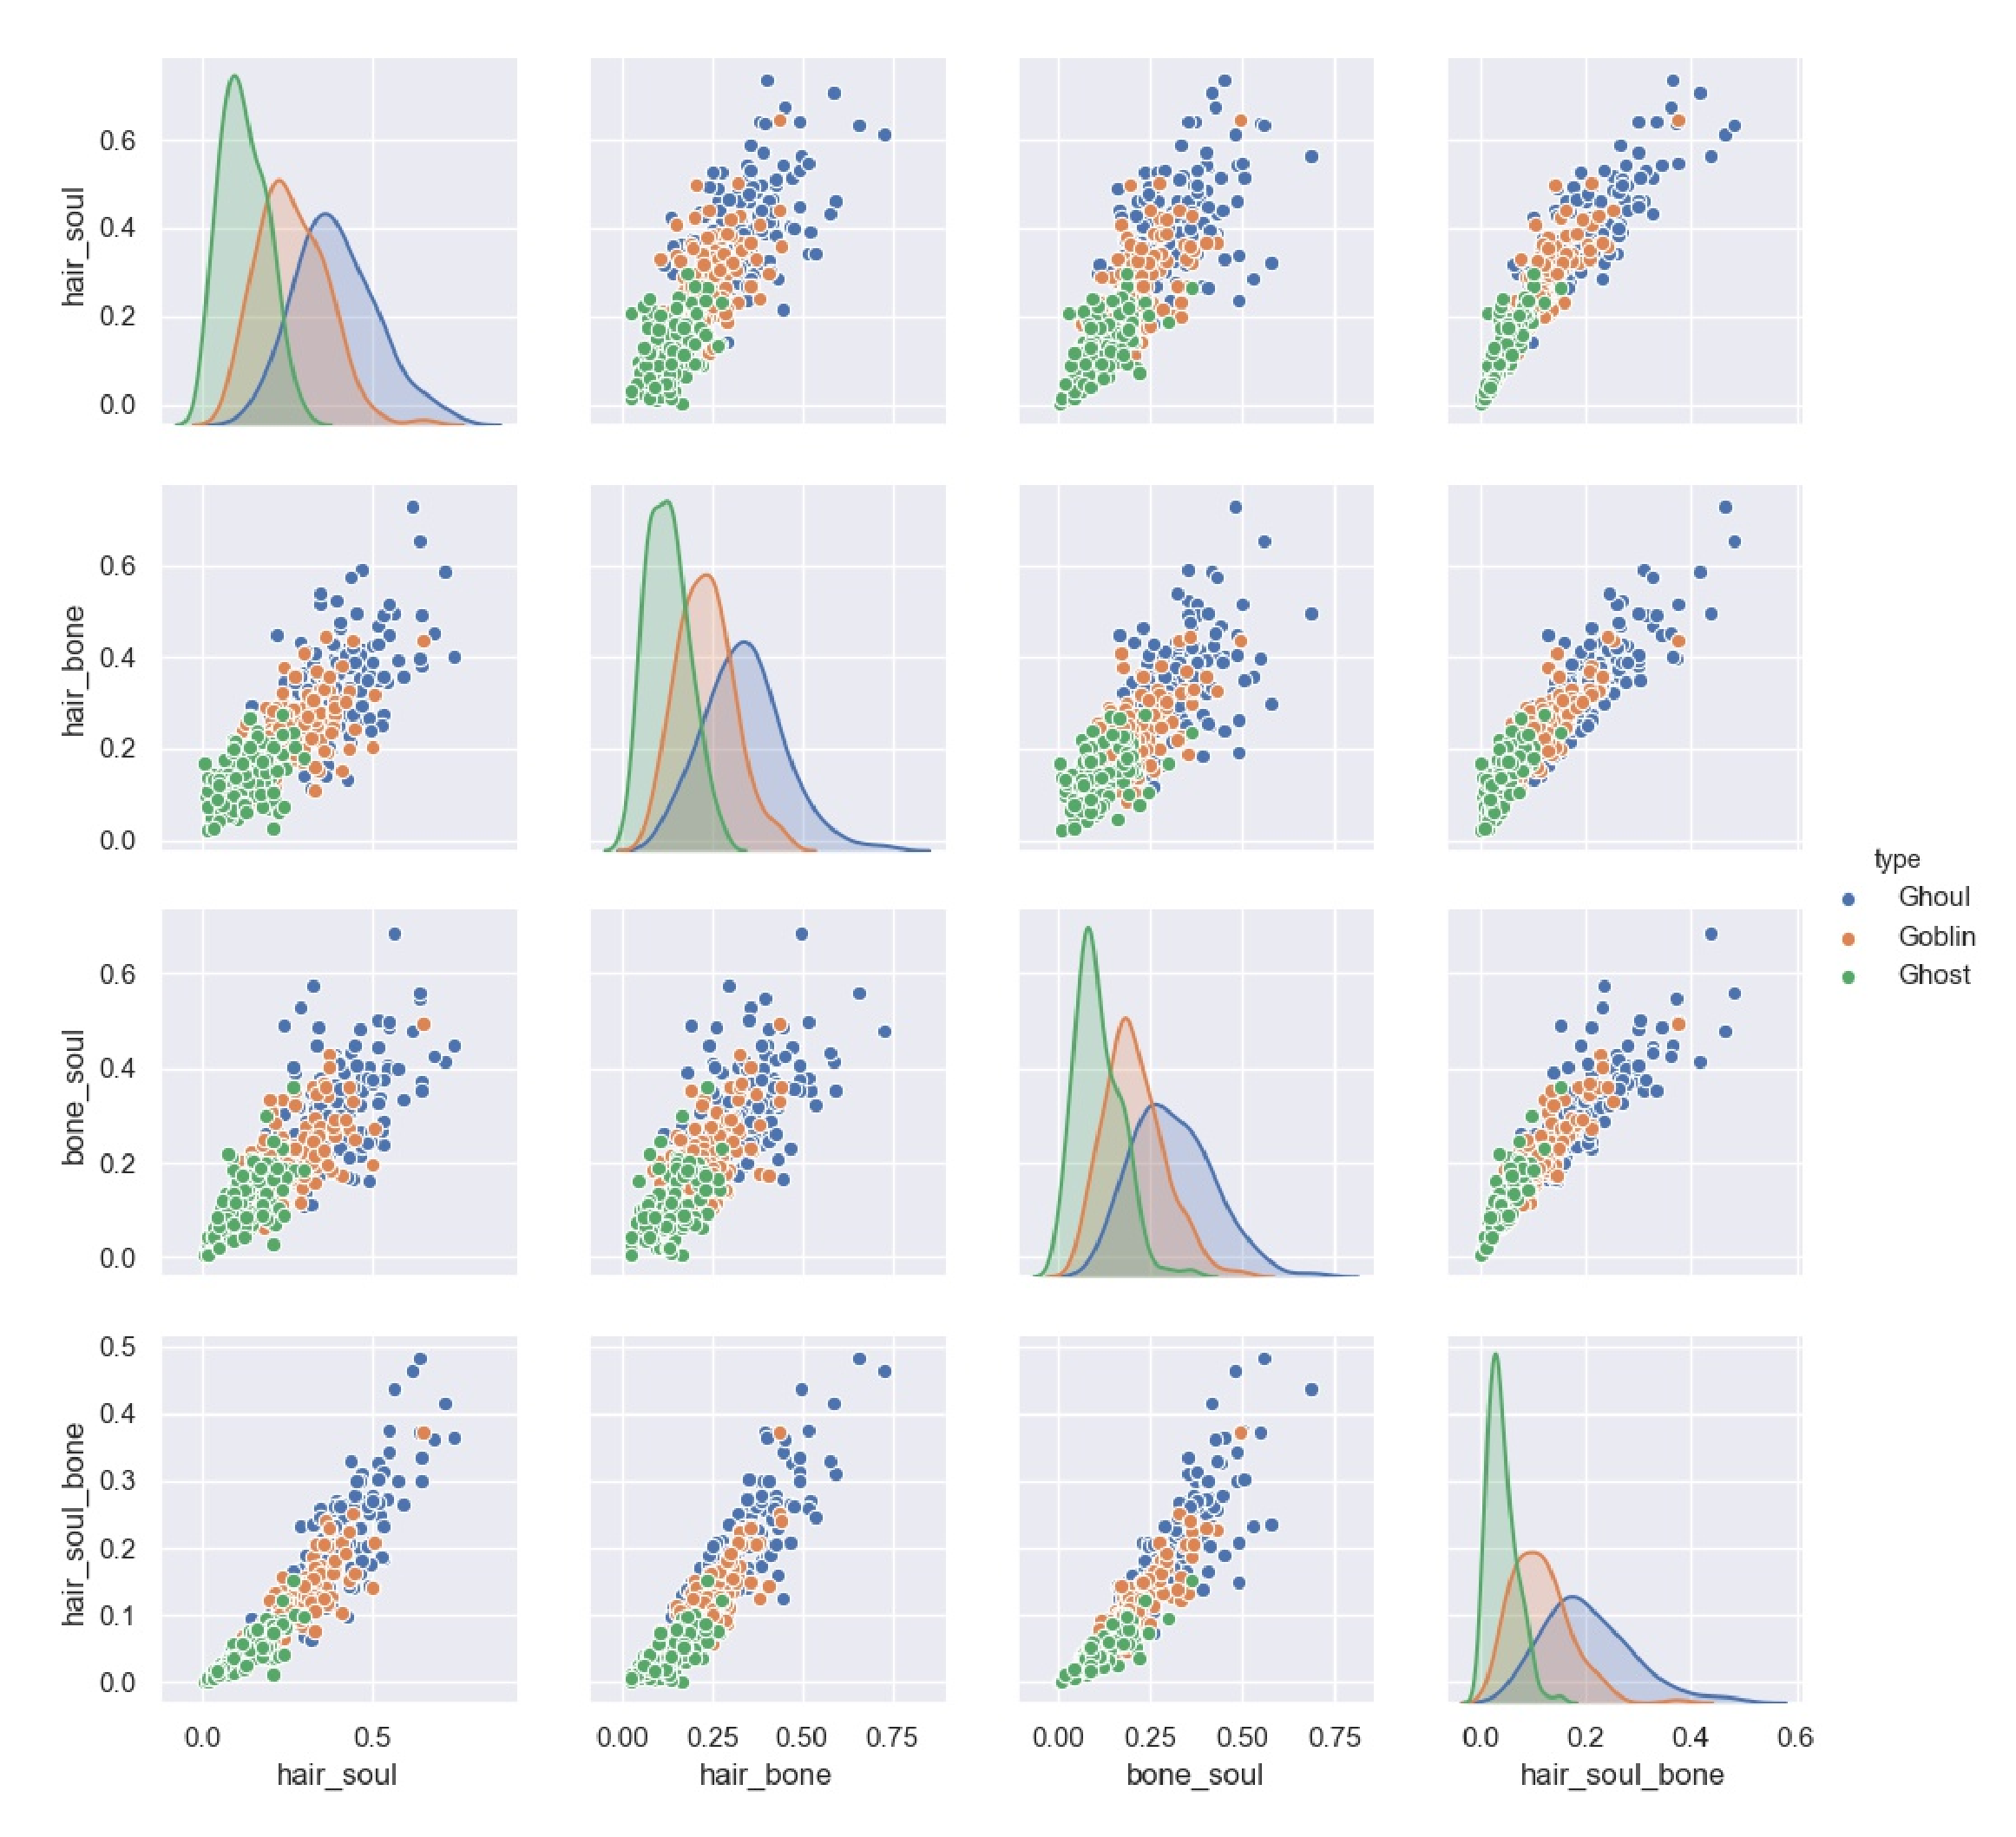
\includegraphics[width=.5\linewidth]{figures/hist_1.eps}
	\end{center}
	
\end{slide}

%%=============================================================

\begin{slide}[toc=,bm=]{New Train Data}
	
	The following figure is 
	a histogram ordered by 
	feature importance. 
	We take the top seven features 
	with higher importance 
	to form a new train data, 
	the rest are discarded.
	\begin{center}
		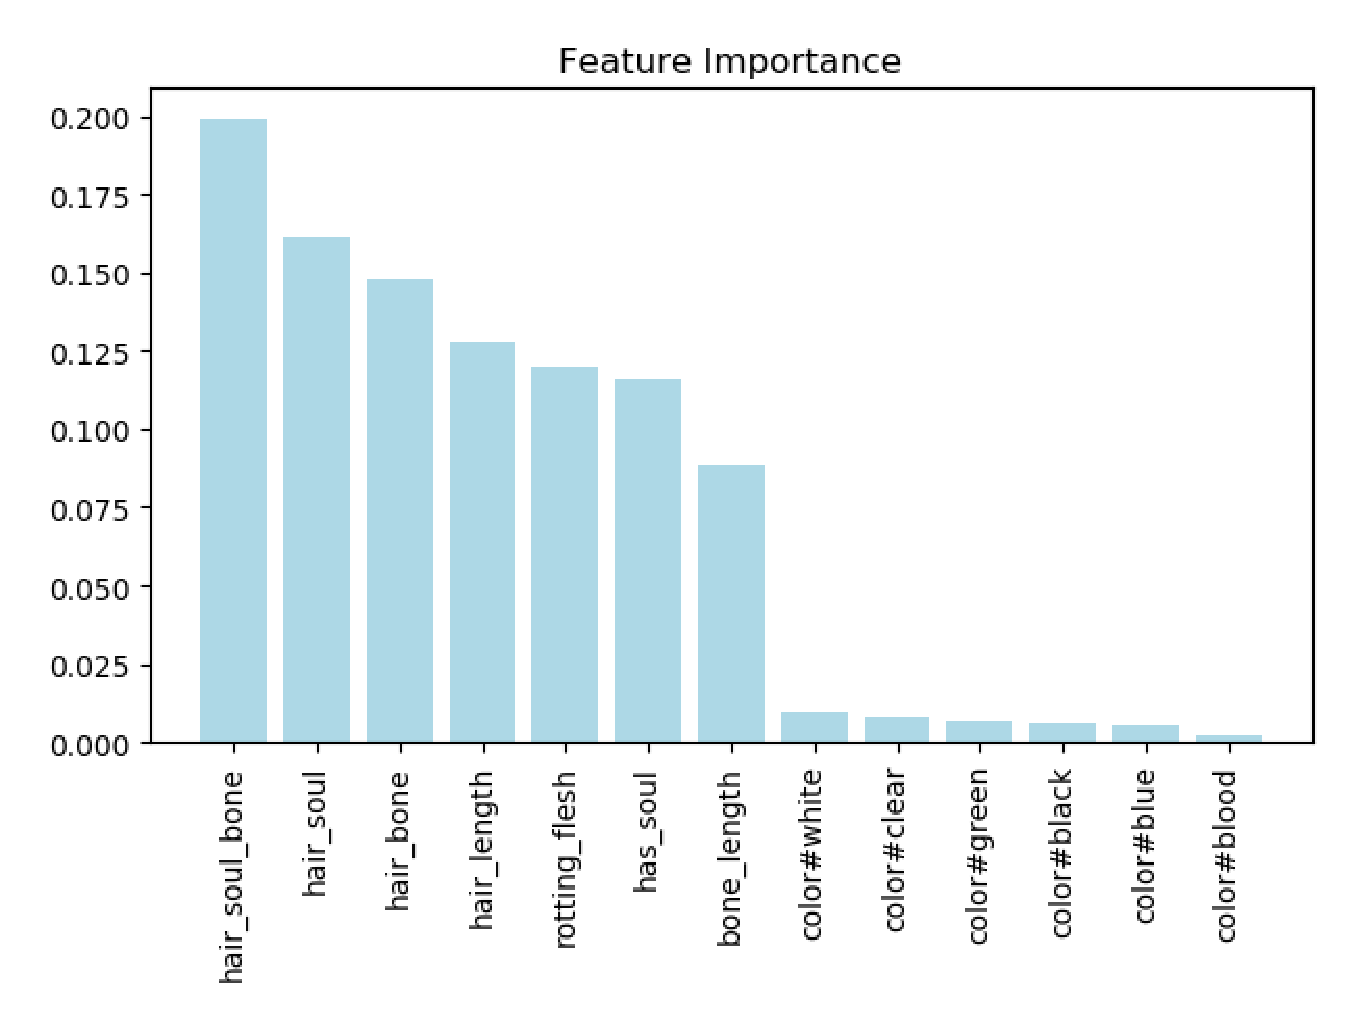
\includegraphics[scale=0.5]{figures/FEATURE.eps}
	\end{center}
	
\end{slide}

%%=============================================================

\section{Methods}


%%==========================================================================================
%%
\begin{slide}{Methods}

There are many machine learning algorithms, 
use the machine learning algorithms below
as Ensemble Model’s base models. 
Through Grid Search and
ten-fold cross-validation
to find the optimal parameters.
Then use the ensemble model on
test data.

\begin{center}
	\begin{itemize}
		\item Base Models
		\
		\begin{itemize}
			\item RandomForeset
			\item LogisticRegression
			\item SVC
			\item KNeighbors
			\item XGBoost
			\item Netual Network
		\end{itemize}
	    \item Ensemble Model
	\end{itemize}
\end{center}

\end{slide}
%%
%%==========================================================================================


\section{Forecast Results}


%%==========================================================================================
%%
\begin{slide}[toc=,bm=]{Forecast Results}
The tables below are 
the metrics classification report 
of ensemble model in 
original and new train data.
\begin{itemize}
	\item Metrics Classification Report of Ensemble Model in original and new train data
\end{itemize}
\begin{center}
	\begin{tabular}{cccccc}
		\hline
		& data &precision & recall & f1-score & support\\
		\hline
		\multirow{2}{*}{Ghost}  & original & 0.80   &   0.83  & 0.82 & 24\\
		& new &0.84  &  0.88  & 0.86 &  24\\
		\hline
		\multirow{2}{*}{Ghoul}  & original & 0.88  &  0.79  &   0.84   &   29\\
		& new & 0.93  & 0.97 &  0.95 &  29\\
		\hline
		\multirow{2}{*}{Goblin}  & original & 0.67  &  0.73 &  0.70  &   22\\
		& new  &  0.80 &  0.73  & 0.76  &  22\\
		\hline  
		multirow{2}{*}{weighted avg}  & original & 0.79  &  0.79 &  0.79  &  75\\
		& new  &  0.86 & 0.87  &  0.86  &  75\\
		\hline 
	\end{tabular}
\end{center}
It can be observed that ensemble model
performaces better in new features.

\end{slide}
%%
%%==========================================================================================


%%
%%==========================================================================================


\section{Conclusion}

%%==========================================================================================
%%
\begin{slide}[toc=,bm=]{Conclusion}
\begin{description}
	\item[Data Exploration] It is an 
	exploratory analysis of the data to 
	provide the necessary conclusions 
	for data processing and modeling.
	\item[Data Preprocessing] This step contains
	dealing with missing data and outliers,
	changing categorical variable 
	into one-hot code and so on.
	\item[Feature Engineering] It's the 
	most important thing.
	Create as more as poosible features,
	then select the most useful features.
	\item[Model Training] The models have 
	many parameters,
	and can use Grid Search to find 
	the optimal paratemers.	
\end{description}



\end{slide}
%%
%%==========================================================================================


%%==========================================================================================
%
\begin{slide}[toc=,bm=]{Questions?}
\begin{center}
\begin{figure}
    \animategraphics[autoplay, loop, height=0.4\textheight]{5}{figures//gif//question//q_}{1}{30}
\end{figure}
\end{center}
\end{slide}
%%
%%==========================================================================================


%%==========================================================================================
% TODO: Contact Page
\begin{wideslide}[toc=,bm=]{Contact Information}
\centering
\vspace{\stretch{1}}
\twocolumn[
lcolwidth=0.35\linewidth,
rcolwidth=0.65\linewidth
]
{
% \centerline{
\includegraphics[scale=.2]{tulip-logo.eps}}
}
{
\vspace{\stretch{1}}
Associate Professor Gang Li\\
School of Information Technology\\
Deakin University, Australia
\begin{description}
 \item[\textcolor{orange}{\faEnvelope}] \href{mailto:gangli@tulip.org.au}
 {\textsc{\footnotesize{gangli@tulip.org.au}}}

 \item[\textcolor{orange}{\faHome}] \href{http://www.tulip.org.au}
 {\textsc{\footnotesize{Team for Universal Learning and Intelligent Processing}}}
\end{description}
}
\vspace{\stretch{1}}
\end{wideslide}

\end{document}

\endinput
